\documentclass[a4paper,10pt]{article}
\usepackage[margin=1in]{geometry}
\usepackage{amsmath}
\usepackage{pgfplots}
\usepackage{amsfonts}
\usepackage{multirow}
\usepackage{graphicx}
\usepackage{caption}
\usepackage{subcaption}
\usepackage{grffile}
\begin{document}
\title{Report}
\maketitle
\section*{Evaluation Data}
16

				\begin{table}[htbp]
				\centering
				\begin{tabular}{|c|c|c|c|}
				\hline
				algorithm&precision&recall&fscore\\
				\hline
				textblocksBS.py&0.2561580101596875&0.6338012365273126&0.34212028271833117\\
VerticalDominance0.py&0.21510660799606252&0.4998219780439376&0.2894479865373125\\
VerticalDominance1.py&0.5445404529358125&0.5239988848800625&0.5197868844554999\\

				\hline
				\end{tabular}
				\end{table}
				 
\section*{Performance Curve}
\begin{figure}[!htbp]
\centering
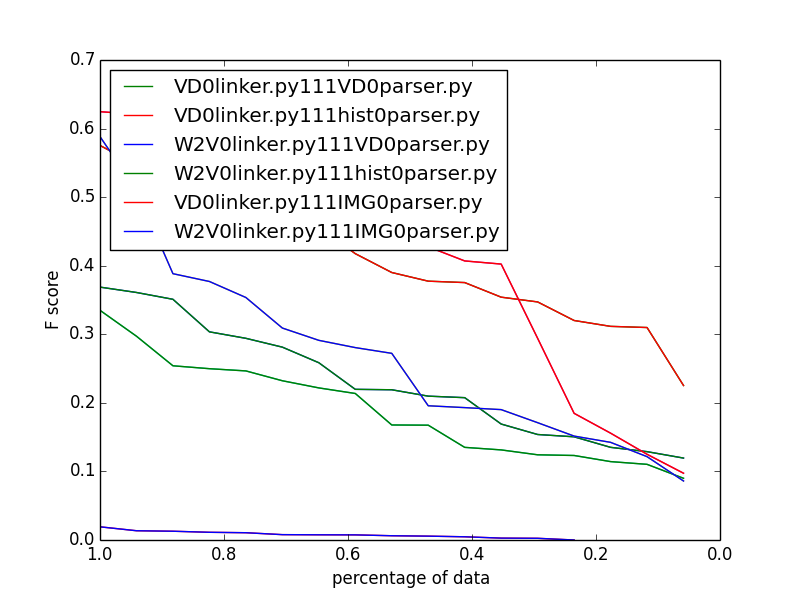
\includegraphics[width = 15cm]{performance.png} 
\end{figure}
\section*{Outliers}
\subsection*{Good outliers}
filter: 0.7

				\begin{table}[htbp]
				\centering
				\begin{tabular}{|c|c|c|}
				\hline
				filename&algorithm&score\\
				\hline
				0003.jpg&VerticalDominance1.py&0.766761768902\\
0005.jpg&VerticalDominance1.py&0.7567104511709999\\

				\hline
				\end{tabular}
				\end{table}
				 
\subsection*{Bad outliers}
filter: 0.4

				\begin{table}[htbp]
				\centering
				\begin{tabular}{|c|c|c|}
				\hline
				filename&algorithm&score\\
				\hline
				0006.jpg&textblocksBS.py&0.287642276423\\
0034.jpg&textblocksBS.py&0.27554027504899997\\
0035.jpg&textblocksBS.py&0.197841726619\\
0037.jpg&textblocksBS.py&0.09658040665429997\\
0038.jpg&textblocksBS.py&0.16970802919699995\\
0045.jpg&textblocksBS.py&0.38719898605800007\\
0259.jpg&textblocksBS.py&0.23276172634900003\\
0292.jpg&textblocksBS.py&0.3526448362719999\\
0296.jpg&textblocksBS.py&0.23367697594499995\\
0003.jpg&VerticalDominance0.py&0.37706475661499994\\
0006.jpg&VerticalDominance0.py&0.288625592417\\
0033.jpg&VerticalDominance0.py&0.39759036144599996\\
0034.jpg&VerticalDominance0.py&0.3502916396629999\\
0035.jpg&VerticalDominance0.py&0.22222222222200003\\
0036.jpg&VerticalDominance0.py&0.33425754775100003\\
0037.jpg&VerticalDominance0.py&0.19999999999999998\\
0038.jpg&VerticalDominance0.py&0.264957264957\\
0045.jpg&VerticalDominance0.py&0.272090777402\\
0253.jpg&VerticalDominance0.py&0.197667087011\\
0255.jpg&VerticalDominance0.py&0.23416391474000003\\
0259.jpg&VerticalDominance0.py&0.262838657501\\
0292.jpg&VerticalDominance0.py&0.13023255814\\
0296.jpg&VerticalDominance0.py&0.20011402508600004\\
0035.jpg&VerticalDominance1.py&0.3703703703699999\\
0037.jpg&VerticalDominance1.py&0.26666666666700006\\
0292.jpg&VerticalDominance1.py&0.193103448276\\

				\hline
				\end{tabular}
				\end{table}
				 
\newpage

					\begin{figure}
					\centering
					\begin{subfigure}{.5\textwidth}
					  \centering
					  \includegraphics[width=10cm]
					{textblocksBS.py.best.png}
					  \caption{best result}
					  \label{fig:sub1}
					\end{subfigure}%
					\begin{subfigure}{.5\textwidth}
					  \centering
					  \includegraphics[width=10cm]
					{textblocksBS.py.gt.best.png}
					  \caption{ground truth}
					  \label{fig:sub2}
					\end{subfigure}
					\caption
					{best result of textblocksBS.py}
					\label{fig:test}
					\end{figure}
					
					\begin{figure}
					\centering
					\begin{subfigure}{.5\textwidth}
					  \centering
					  \includegraphics[width=10cm]
					{textblocksBS.py.worst.png}
					  \caption{worst result}
					  \label{fig:sub1}
					\end{subfigure}%
					\begin{subfigure}{.5\textwidth}
					  \centering
					  \includegraphics[width=10cm]
					{textblocksBS.py.gt.worst.png}
					  \caption{ground truth}
					  \label{fig:sub2}
					\end{subfigure}
					\caption
					{worst result of textblocksBS.py}
					\label{fig:test}
					\end{figure}
					
					\begin{figure}
					\centering
					\begin{subfigure}{.5\textwidth}
					  \centering
					  \includegraphics[width=10cm]
					{VerticalDominance0.py.best.png}
					  \caption{best result}
					  \label{fig:sub1}
					\end{subfigure}%
					\begin{subfigure}{.5\textwidth}
					  \centering
					  \includegraphics[width=10cm]
					{VerticalDominance0.py.gt.best.png}
					  \caption{ground truth}
					  \label{fig:sub2}
					\end{subfigure}
					\caption
					{best result of VerticalDominance0.py}
					\label{fig:test}
					\end{figure}
					
					\begin{figure}
					\centering
					\begin{subfigure}{.5\textwidth}
					  \centering
					  \includegraphics[width=10cm]
					{VerticalDominance0.py.worst.png}
					  \caption{worst result}
					  \label{fig:sub1}
					\end{subfigure}%
					\begin{subfigure}{.5\textwidth}
					  \centering
					  \includegraphics[width=10cm]
					{VerticalDominance0.py.gt.worst.png}
					  \caption{ground truth}
					  \label{fig:sub2}
					\end{subfigure}
					\caption
					{worst result of VerticalDominance0.py}
					\label{fig:test}
					\end{figure}
					
					\begin{figure}
					\centering
					\begin{subfigure}{.5\textwidth}
					  \centering
					  \includegraphics[width=10cm]
					{VerticalDominance1.py.best.png}
					  \caption{best result}
					  \label{fig:sub1}
					\end{subfigure}%
					\begin{subfigure}{.5\textwidth}
					  \centering
					  \includegraphics[width=10cm]
					{VerticalDominance1.py.gt.best.png}
					  \caption{ground truth}
					  \label{fig:sub2}
					\end{subfigure}
					\caption
					{best result of VerticalDominance1.py}
					\label{fig:test}
					\end{figure}
					
					\begin{figure}
					\centering
					\begin{subfigure}{.5\textwidth}
					  \centering
					  \includegraphics[width=10cm]
					{VerticalDominance1.py.worst.png}
					  \caption{worst result}
					  \label{fig:sub1}
					\end{subfigure}%
					\begin{subfigure}{.5\textwidth}
					  \centering
					  \includegraphics[width=10cm]
					{VerticalDominance1.py.gt.worst.png}
					  \caption{ground truth}
					  \label{fig:sub2}
					\end{subfigure}
					\caption
					{worst result of VerticalDominance1.py}
					\label{fig:test}
					\end{figure}
					
\end{document}